\documentclass[11pt,letterpaper]{article}

% be able to include figures
\usepackage{graphicx}
% get nice colors
\usepackage{xcolor}

% change default font to Palatino (looks nicer!)
\usepackage[latin1]{inputenc}
\usepackage{mathpazo}
\usepackage[T1]{fontenc}
% load some useful math symbols/fonts
\usepackage{latexsym,amsfonts,amsmath,amssymb}

% comfort package to easily set margins
\usepackage[top=1in, bottom=1in, left=1in, right=1in]{geometry}

% control some spacings
%
% spacing after a paragraph
\setlength{\parskip}{.15cm}
% indentation at the top of a new paragraph
\setlength{\parindent}{0.0cm}


\begin{document}

\begin{center}
\Large
Ay190 -- Worksheet 2\\
Daniel DeFelippis\\
Date: \today
\end{center}

%%
%%
%% I worked with Scott Barenfeld
%%
%%

\section{}
Implementing the recurrence relationship 
$$x_n = \frac{13}{3}x_{n-1} - \frac{4}{3}x_{n-2},$$ 
equivalent to $x_n = \left(\frac{1}{3}\right)^{n}$, 
to find $x_{15}$ for $x_0 = 1, x_1 = \frac{1}{3}$ 
using single precision (float32) numbers in python, we get that $x_{15} = 3.65749$. 
This is obviously very different from the answer found simply computing
$\left(\frac{1}{3}\right)^{15}$ using double precision (float64) numbers, $6.96917193763*10^{-8}$.

The absolute and relative errors are $-3.6574$ and $-52481030.9737$ 
respectively, which goes to show how differently single precision floating
point numbers can behave from double precision ones.

\section{}


We discretize the function $f(x) = x^3 - 5x^2 + x$ on the interval $[-2, 6]$
and compute the derivative using forward differencing, given by 
$$f'(x) = \frac{f(x+h) - f(x)}{h} + \mathcal{O}(h)$$ and central 
differencing, given by 
$$f'(x) = \frac{f(x+h) - f(x-h)}{2h} + \mathcal{O}(h^2)$$

\begin{figure}[bth]
\centering
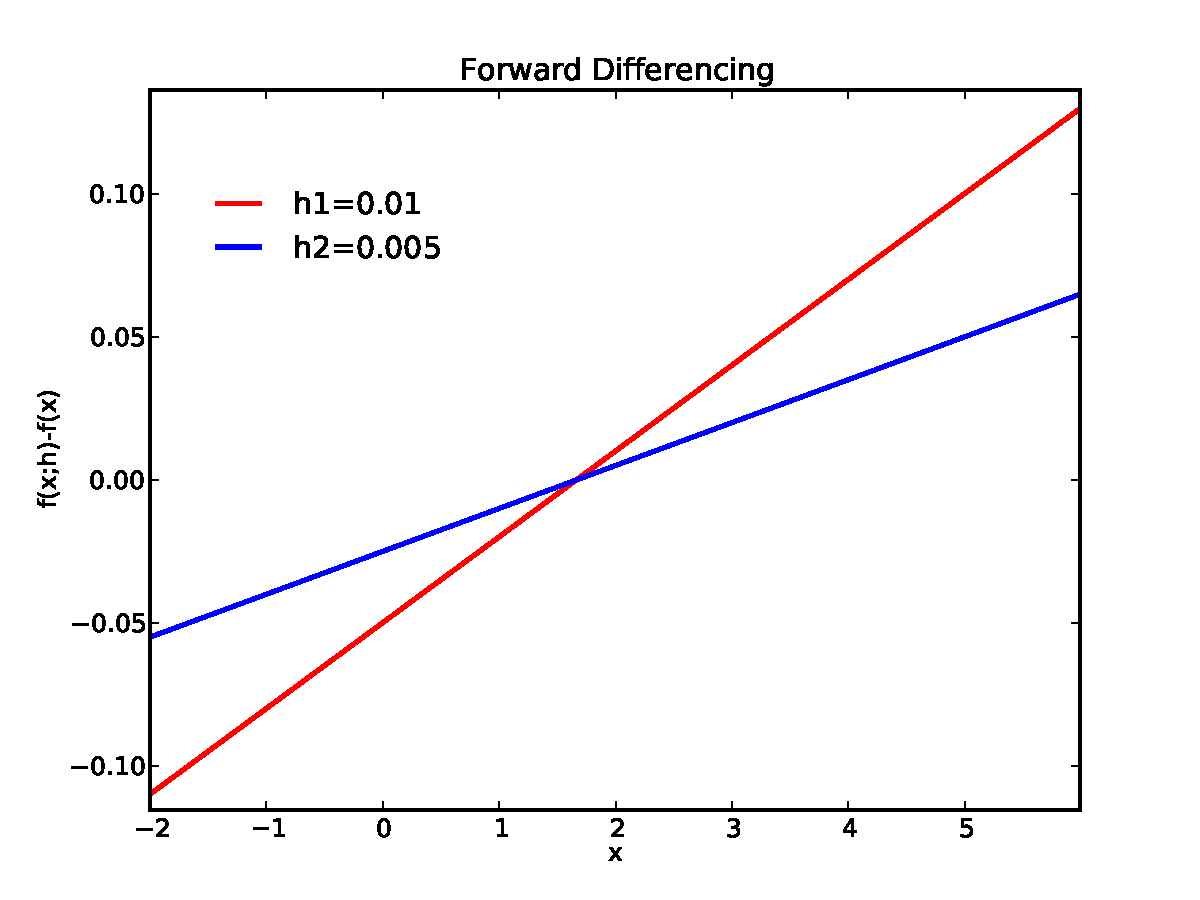
\includegraphics[width=0.5\textwidth]{forward_differencing.pdf}
\caption{Error of forward differencing with steps sizes $h_1 > h_2$}
\label{fig:forward}
\end{figure}

We use two step sizes, $h_1 = 0.01$ and $h_2 = h_1/2 = 0.005$. 
Plotting the error of the forward differencing, it is clear from figure~\ref{fig:forward} that 
the smaller step size produces the smaller error.

Furthermore, we see that at every x, the error of h2 is half of that of h1, 
which means that since the convergence factor
$Q = \left(\frac{h_2}{h_1}\right)^{n} = \frac{1}{2}$, 
$\left(\frac{h_2}{h_1}\right)^{n} = \left(\frac{0.005}{0.01}\right)^n = \frac{1}{2} 
\Rightarrow n = 1$. So, forward differencing is first-order convergent.

\begin{figure}[bth]
\centering
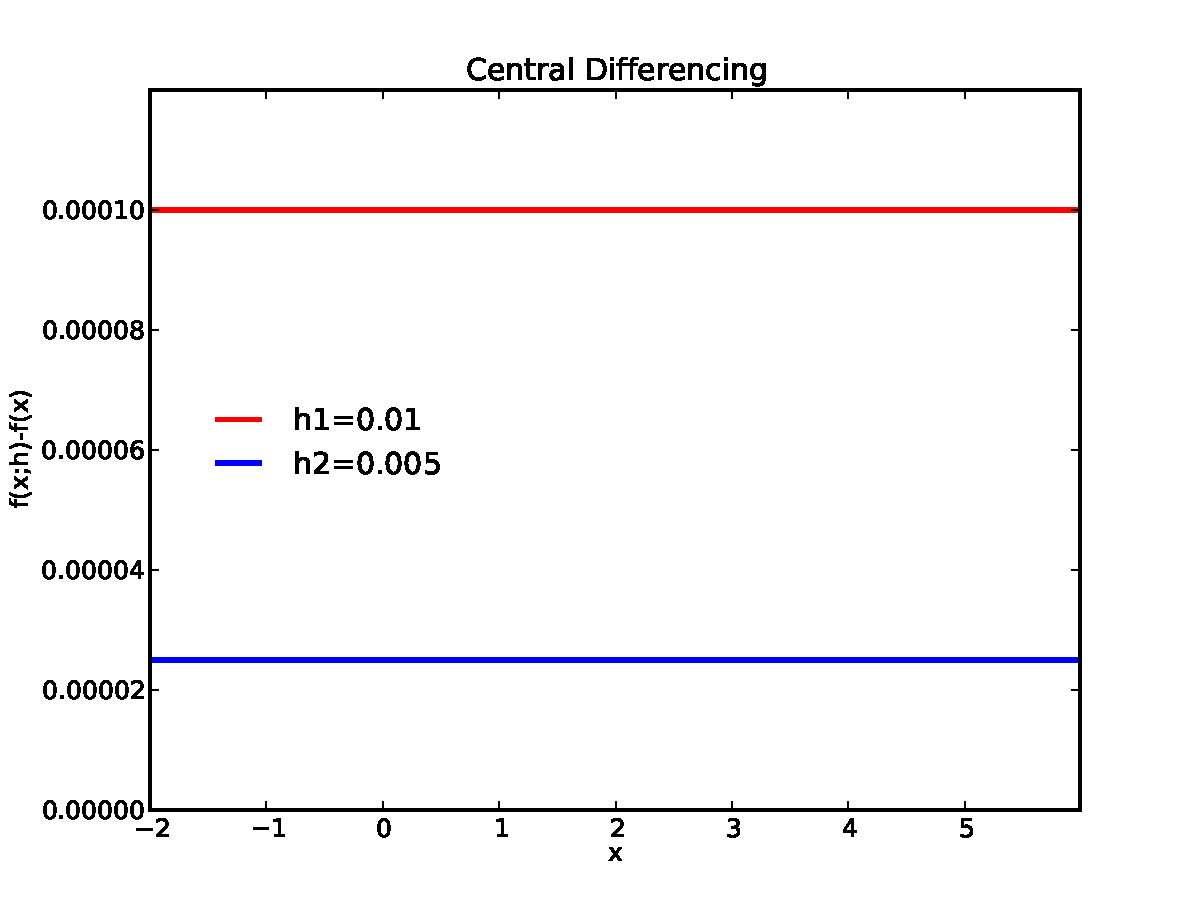
\includegraphics[width=0.5\textwidth]{central_differencing.pdf}
\caption{Error of central differencing with steps sizes $h_1 > h_2$}
\label{fig:central}
\end{figure}

In figure~\ref{fig:central}, we see that the overall error for central 
differencing is many orders of magnitude smaller than the forward differencing.
We also see that, with the same step sizes, the quality of the convergence 
increases by more than a factor of 2: it increases by a factor of 4. This means,
using the formula for Q above, $\left(\frac{0.005}{0.01}\right)^n = \frac{1}{4} 
\Rightarrow n = 2$. So, central differencing is second-order convergent.

\section{}
We use the Taylor expansion of $f(x_0+h)$ given in the notes as formula (III.2.2):
$$f(x_0+h) = \sum\limits_{n=0}^{\infty} \frac{f^{(n)}(x_0)}{n!}h^n = 
f(x_0) + hf'(x_0) + \frac{h^2}{2}f''(x_0) + \frac{h^3}{6}f'''(x_0) 
+ \frac{h^4}{24}f''''(x_0) + \mathcal{O}(h^5)$$
Note that, if we replace $h$ with $-h$, the odd powers of $h$ change signs 
in the expression above, so we also have 
$$f(x_0-h) = \sum\limits_{n=0}^{\infty} \frac{f^{(n)}(x_0)}{n!}h^n = 
f(x_0) - hf'(x_0) + \frac{h^2}{2}f''(x_0) - \frac{h^3}{6}f'''(x_0) 
+ \frac{h^4}{24}f''''(x_0) - \mathcal{O}(h^5)$$.
Adding these two equations together and solving for $f''(x_0)$ gives
$$f''(x_0) = \frac{f(x_0+h) + f(x_0-h) - 2f(x_0)}{h^2} - \frac{h^2}{12}f''''(x_0) - \mathcal{O}(h^4)$$
If we neglect the fourth derivative, then we have found a central difference
approximation that is second order in h:
$$f''(x_0) = \frac{f(x_0+h) -2f(x_0) + f(x_0-h)}{h^2}  - \mathcal{O}(h^2)$$


\section{}
In this problem, we interpolate the 9 data points using first a global
Lagrane interpolation, then piecewise linear and quadratic interpolations.
The plots are shown below.
\subsection*{a}

\begin{figure}[bth]
\centering
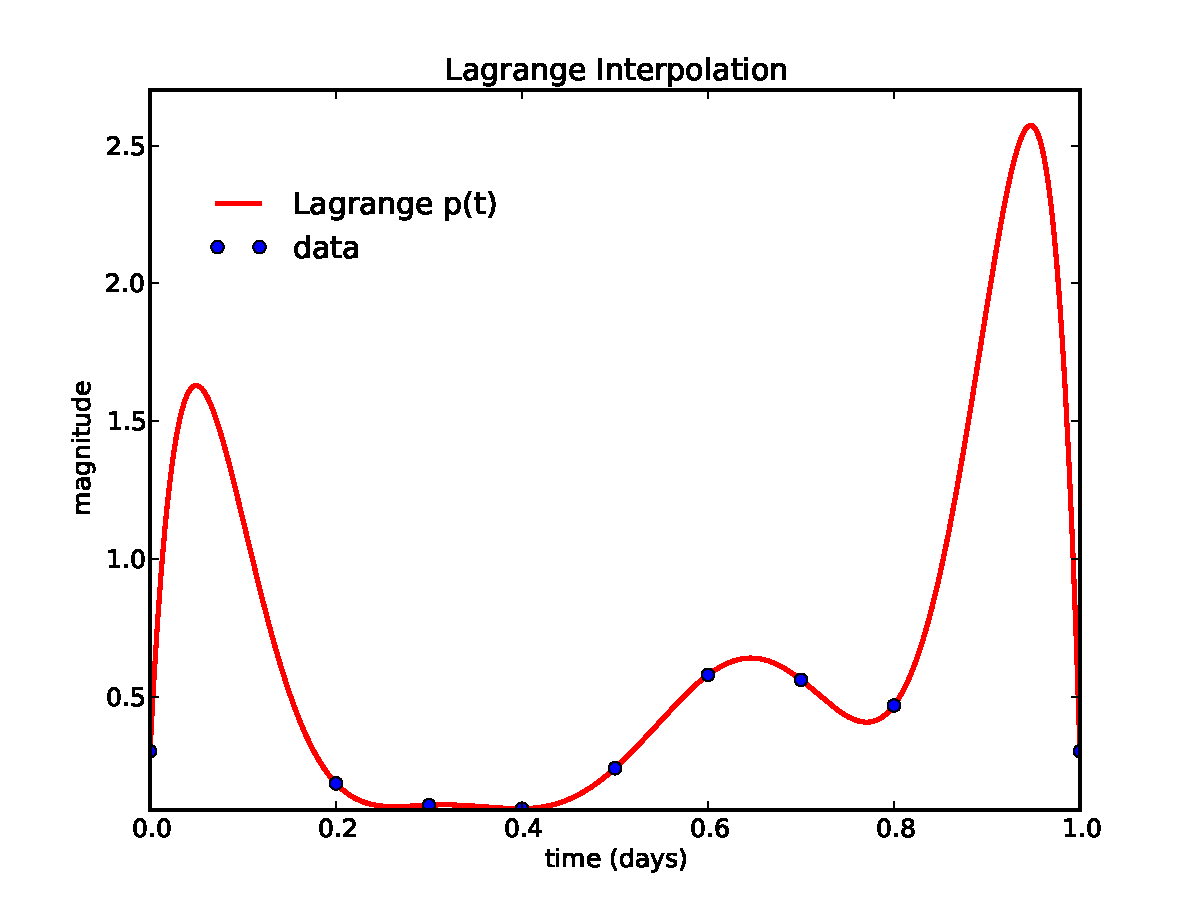
\includegraphics[width=0.5\textwidth]{lagrange_interpolation.pdf}
\caption{Lagrange interpolation polynomial of degree 8 with Cepheid data}
\label{fig:lagrange}
\end{figure}

The polynomial smoothly connects the middle points, but between the first and 
last two points, it jumps wildly, demonstrating that higher order polynomials
aren't necessarily better since large oscillations may develop.

\subsection*{b}

\begin{figure}[bth]
\centering
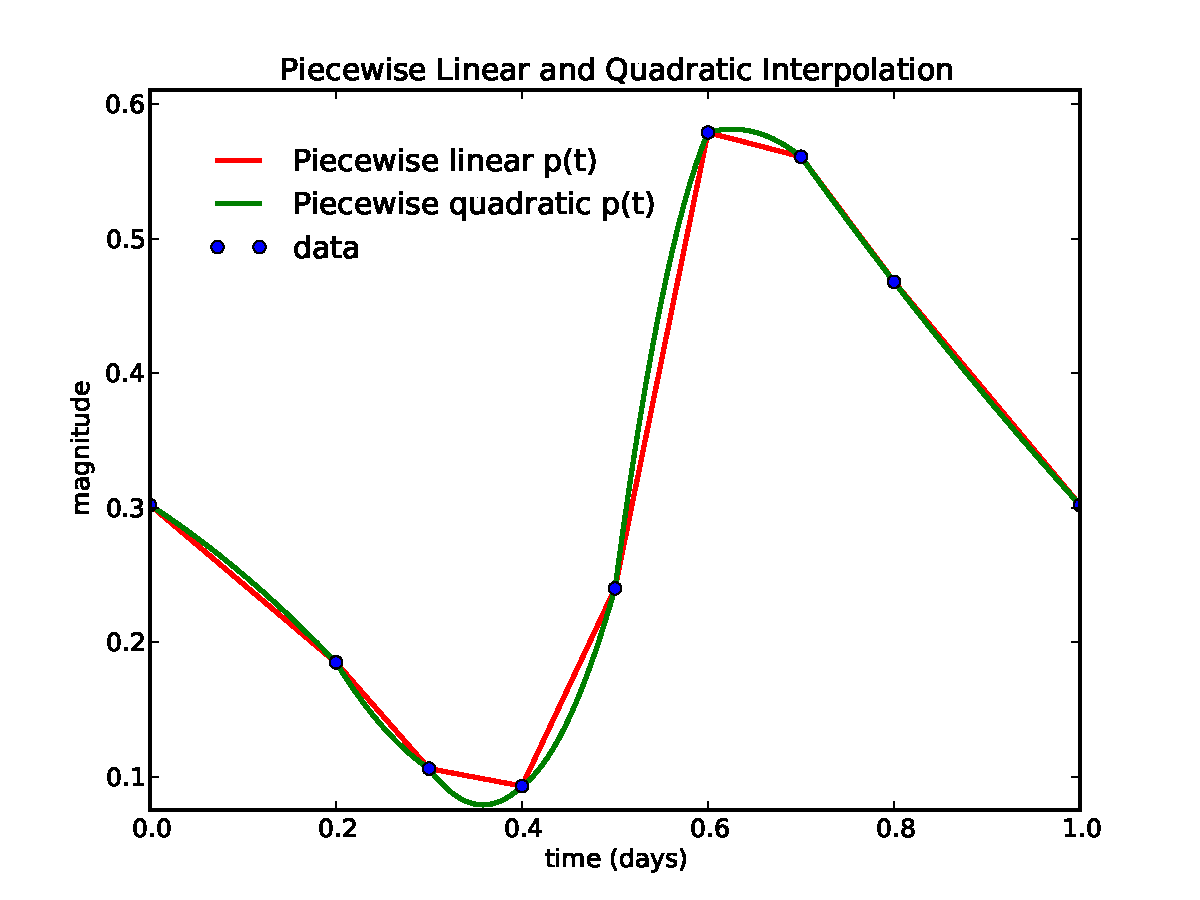
\includegraphics[width=0.5\textwidth]{linear_and_quadratic_interpolation.pdf}
\caption{Piecewise linear and quadratic interpolations with Cepheid data}
\label{fig:lin-quad}
\end{figure}

The piecewise interpolations work better over the entire range of data,
avoiding the oscillatory behavior of the global interpolation in figure~\ref{fig:lagrange}. Plotting the three interpolations together, as in 
figure~\ref{fig:lin-quad-lag} demonstrates just how better the piecewise 
interpolations capture the data.

\begin{figure}[bth]
\centering
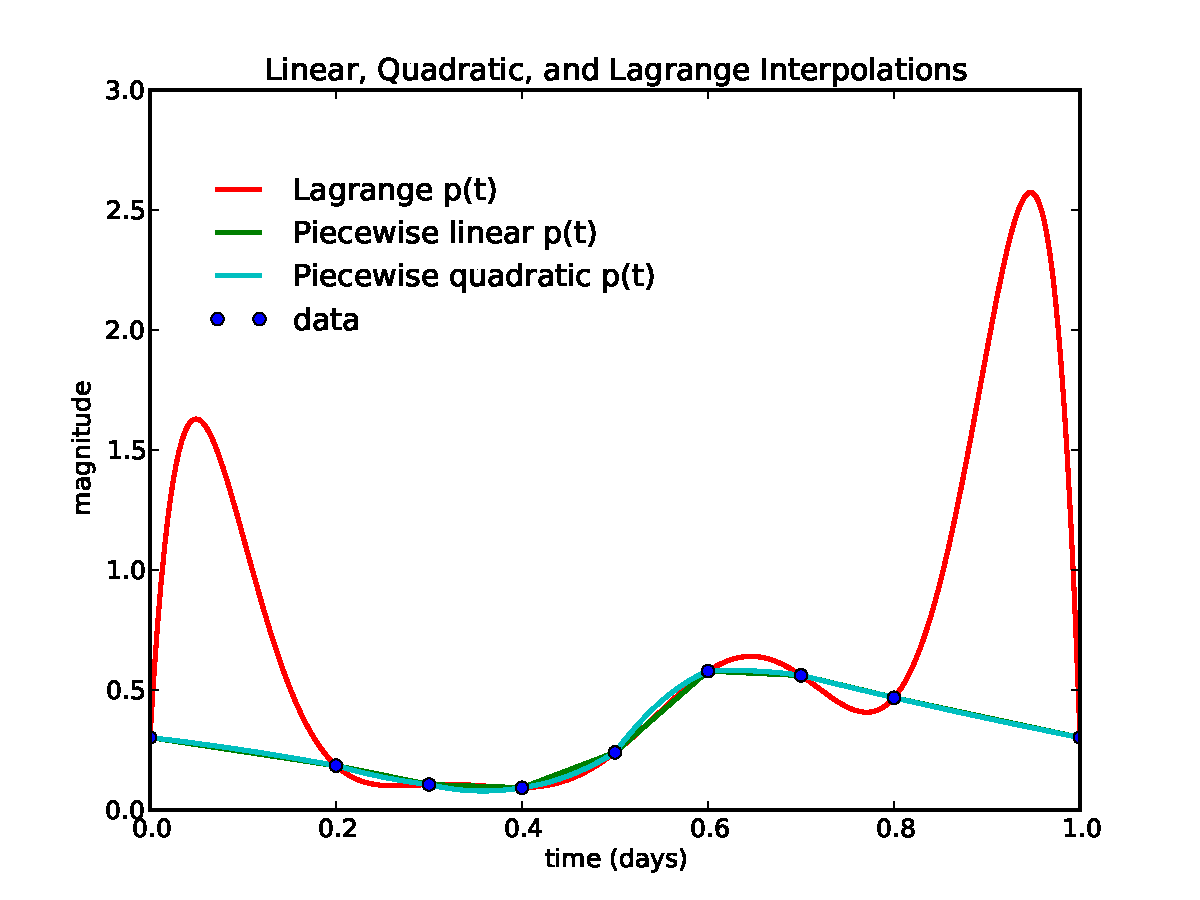
\includegraphics[width=0.5\textwidth]{linear_quadratic_lagrange_interpolation.pdf}
\caption{Piecewise linear and quadratic interpolations with Cepheid data}
\label{fig:lin-quad-lag}
\end{figure}

\section{}
Piecewise cubic Hermite interpolation, and then a natural cubic spline 
interpolation.

\subsection*{a}

\begin{figure}[bth]
\centering
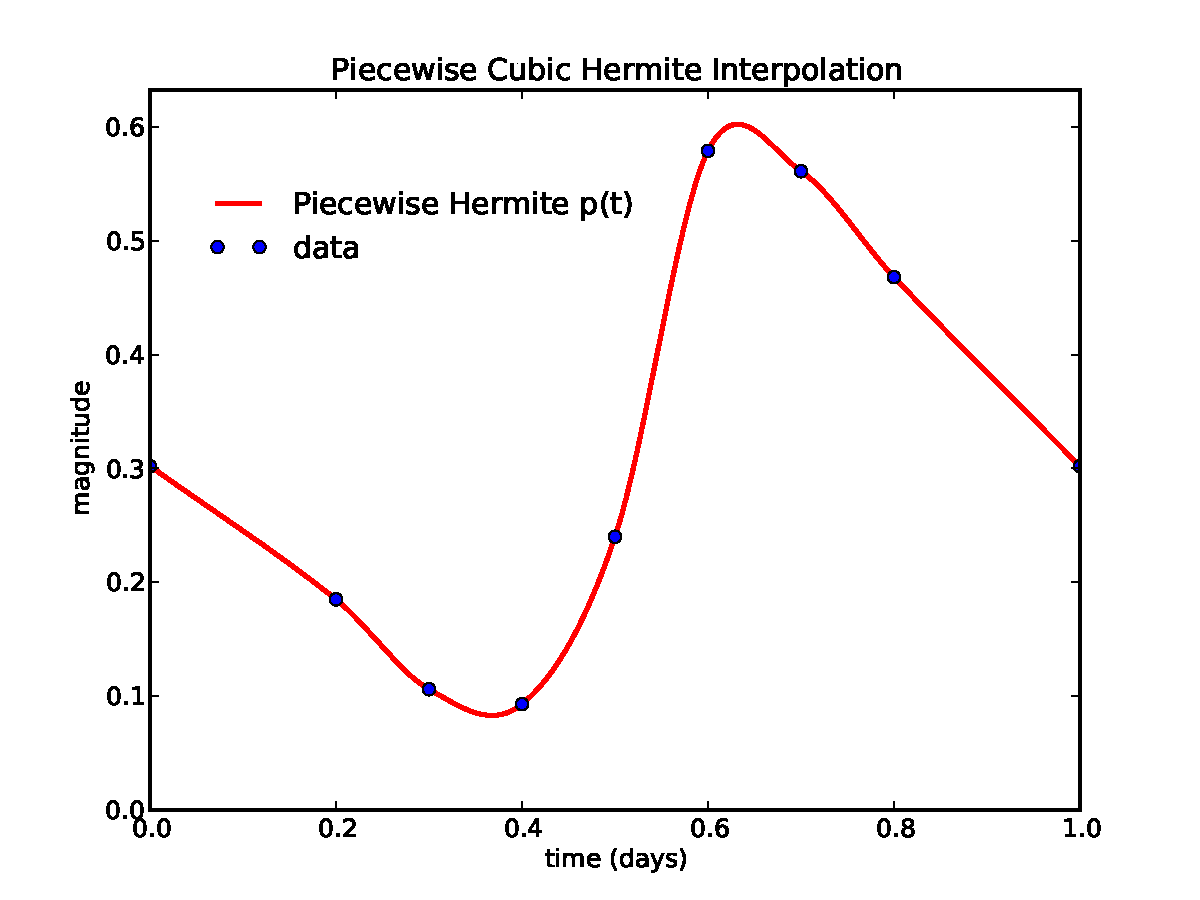
\includegraphics[width=0.5\textwidth]{hermite_interpolation.pdf}
\caption{Piecewise cubic Hermite interpolation with Cepheid data}
\label{fig:hermite}
\end{figure}


\subsection*{b}

\begin{figure}[bth]
\centering
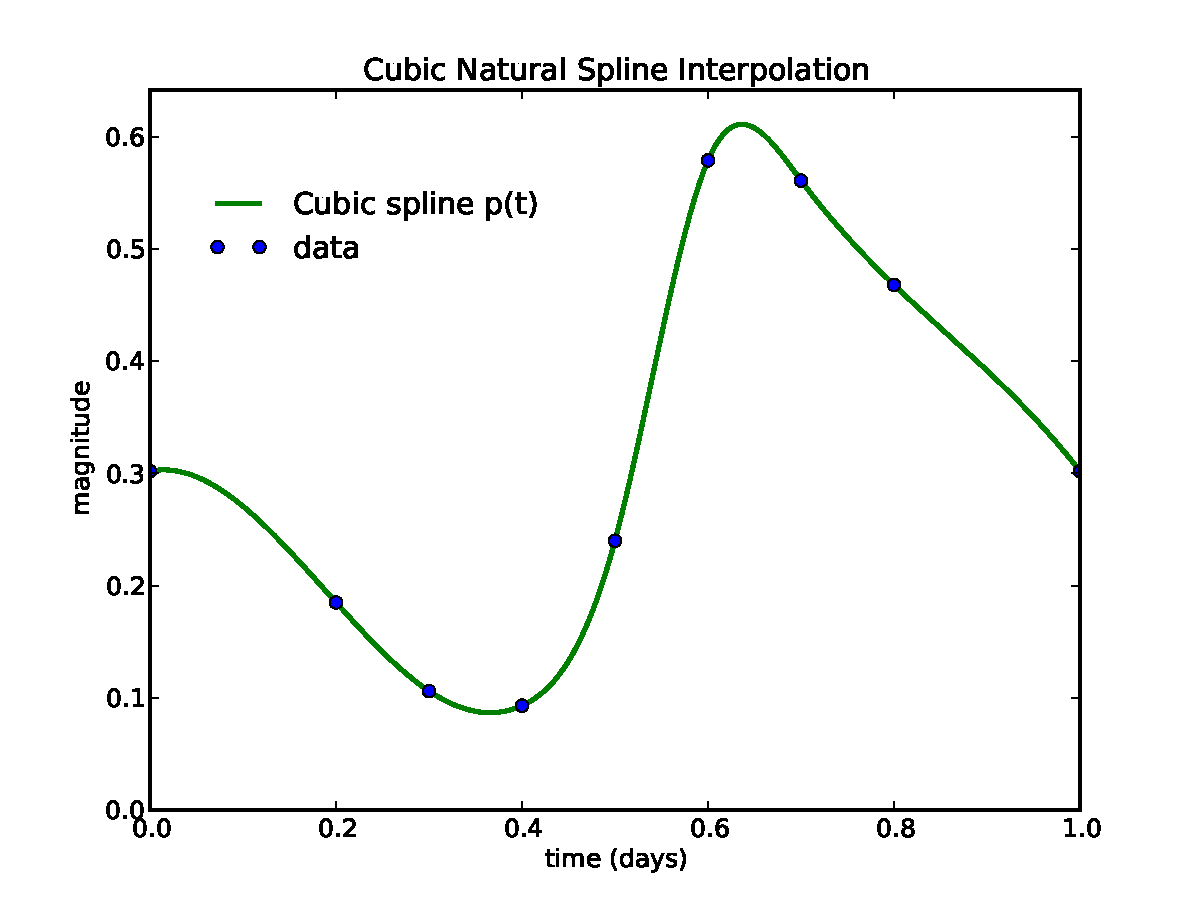
\includegraphics[width=0.5\textwidth]{spline_interpolation.pdf}
\caption{Cubic natural Spline interpolation with Cepheid data}
\label{fig:spline}
\end{figure}

Comparing the hermite and spline interpolations on the same plot,
figure~\ref{fig:herm-spl}, some differences become clear. The spline plot 
in between $t=0$ and $t=0.2$ is much more curved than the hermite one, which is
essentially linear. In general, the spline plot is smoother with more
rounded peaks than the hermite plot.

\begin{figure}[bth]
\centering
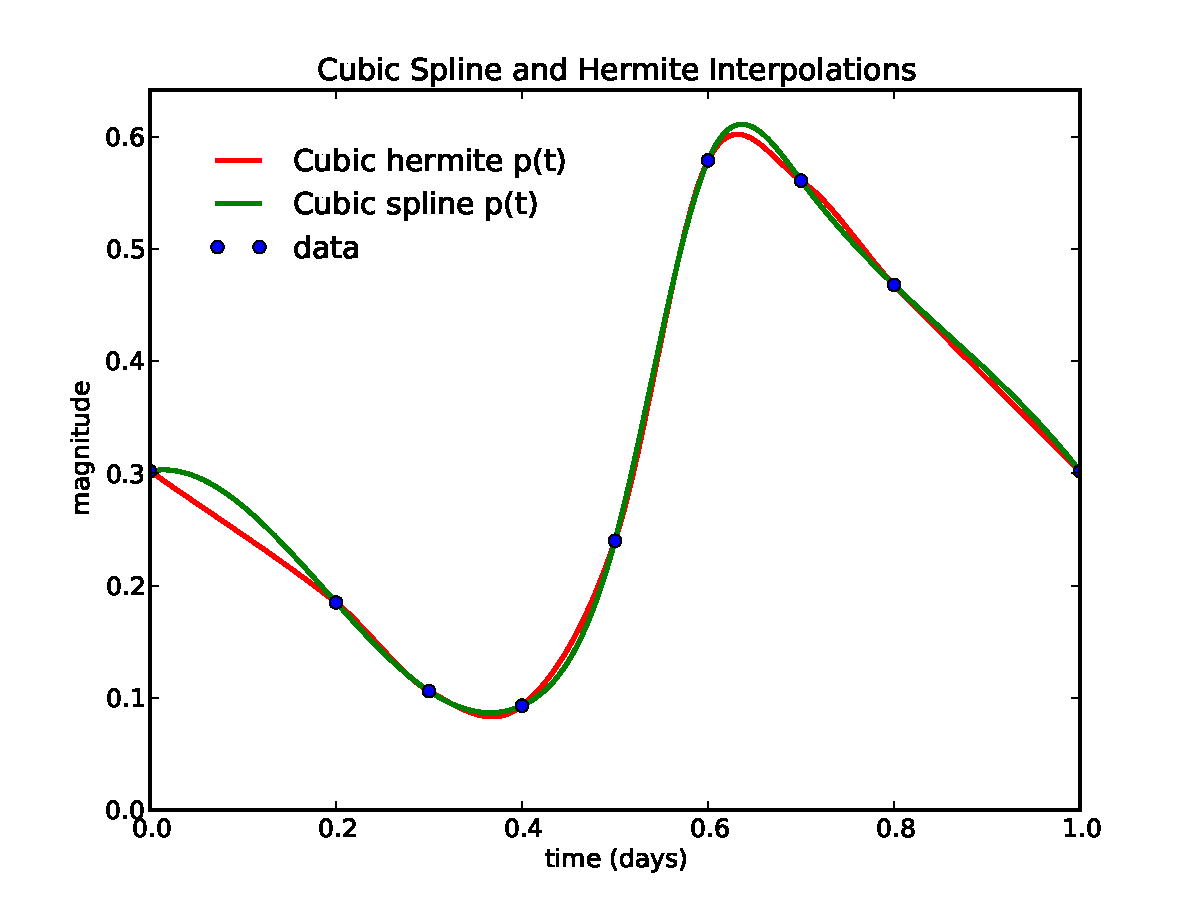
\includegraphics[width=0.5\textwidth]{hermite_spline_interpolation.pdf}
\caption{Cubic Spline and Hermite interpolations with Cepheid data}
\label{fig:herm-spl}
\end{figure}




*Code for all of the results and plots are found in my git repository under
ws2.*
\end{document}
